\documentclass[a4paper, titlepage]{report}

\usepackage[utf8]{inputenc}
\usepackage[french]{babel}
\usepackage[T1]{fontenc}
\usepackage{geometry}         % marges
\usepackage{graphicx}         % images
\usepackage{verbatim}         % texte préformaté
\usepackage{url}
\usepackage{listings}
\usepackage{multicol}
\usepackage[font=small,labelfont=bf]{caption}
\usepackage{subfiles}
\usepackage{tikz}
\usepackage[parfill]{parskip}
\usetikzlibrary{positioning, quotes}

\renewcommand{\lstlistingname}{Programme}% Listing -> Algorithm
\renewcommand{\lstlistlistingname}{Liste de \lstlistingname s}% List of Listings -> List of Algorithms



\title{Rapport projet Cassiopée 93\\ \large Structural souce code properties}      % renseigne le titre
\author{Julien DENIZE \and Cyprien LAMBERT \\ \and Tuteur: Jorge-Eleazar LOPEZ-CORONADO}           %   "   "   l'auteur
\date{29 mai 2019}           %   "   "   la future date de parution

\begin{document}

\begin{titlepage}
    \parindent=0pt
    Cassiopée 2019: projet 93 \hspace*{\stretch{1}}
    \vspace*{\stretch{1}}
    \begin{center}\bfseries\Huge
        Structural source code properties
    \end{center}
    \vspace*{1cm}
    \begin{center}
        
\includegraphics[scale=0.2]{images/iconcassiopee}
        
\includegraphics[scale=0.81]{images/tsp}
        \end{center}
    \begin{center}\bfseries\Large
    Julien DENIZE - Cyprien LAMBERT
    \end{center}
        
    \begin{center}\bfseries\Large
    Sous la direction de Jorge-Eleazar LOPEZ-CORONADO.
    \end{center}
    \vspace*{\stretch{2}}
    \begin{flushright}
            Le \today 
    \end{flushright}
\end{titlepage}
\tableofcontents

% --- inserer votre code LaTeX ici ---

\chapter{Introduction} 
\section{Qu'est ce que l'optimisation}
\subsection{Définition}
Selon la définition donnée par Wikipédia:
\begin{quote}
    En programmation informatique, l'optimisation de code est la pratique consistant à améliorer l'efficacité du code informatique ou d'une librairie logicielle. \cite{wiki:Optimisation_de_code}
\end{quote}
Ainsi l'optimisation en informatique fait partie intégrante du développement. En effet, il est crucial pour différentes raisons détaillés à la section suivante que les développeurs optimisent leur code afin d'améliorer son rendement.

Des recherches ont donc été effectuées durant de nombreuses années au début de l'informatique afin d'optimiser le compilateur par exemple, pour avoir des compilations plus rapides ou/et plus efficaces. Aujourd'hui encore, la rercheche en optimisation est importante car mêmes si les machines sont de plus en plus puissantes, les algorithmes sont de plus en plus gourmands également.

Le Big Data illustre parfaitement ceci, les machines peuvent traiter des millions et des millions de données, mais si les algorithmes mettent des mois à s'exécuter, alors cela aurait eu peu de valeur.

\subsection{Problèmes à résoudre par optimisation}
Les optimisations permettent d'améliorer nombreuses choses: une exécutions plus rapide, une place en mémoire réduite, une limitation des ressources consommées comme les fichiers et enfin une diminution de la consommation électrique.

En effet, les optimisations permettent de supprimer des choses inutiles par exemple le code suivant:
\newpage
\begin{center}
\begin{lstlisting}[language=c, xleftmargin=.35\textwidth, caption={Exemple de code non optimisé}, captionpos=b]
int foo(const int d) {
    int a = d;
    int b = 1 + a;
    return b;
}
\end{lstlisting}
\end{center}
pourrait être optimisé de la façon suivante:
\begin{lstlisting}[language=c, xleftmargin=.35\textwidth, caption={Exemple de code optimisé}, captionpos=b]
int foo(const int d) {
    return 1 + d;
}
\end{lstlisting}
Cette "simple" optimisation permet de répondre aux différents critères d'amélioration. Le code est plus rapide, plus court donc il prend moins de place en mémoire, consomme moins d'énergie et enfin il utilise moins de ressources en RAM.

\subsection{Outils existants}
De très nombreux outils plus ou moins connus sont dédiés à l'optimisation de code, et ce dans tous les languages de programmation. La bibliothèque de compilation GCC\footnote{GCC (GNU Compiler Collection) est une suite de logiciels libres de compilation. On l'utilise dans le monde Linux dès que l'on veut transcrire du code source en langage machine, c'est le plus répandu des compilateurs. - \url{https://doc.ubuntu-fr.org/gcc}}, par exemple permet à l'utilisateur d'appliquer facilement nombre d'optimisations à son code. L'optimisation présentée à la section précédente est possible via GCC.

Les outils procèdent généralement à une analyse statique du code afin de l'optimiser ou de signaler des erreurs aux programmeurs. Cela signifie que le programme analysé n'est pas exécuté mais que les outils procèdent à une analyse syntaxique du programme afin d'étudier sa structure. L'analyse dynamique, avec exécution du programme, est d'avantage utilisée pour faire des tests afin de vérifier que le programme répond à des spécifications.  


\section{Notre approche}
\subsection{Les Control Flow Graphs (CFG)}
Nous nous sommes d'abord concentrés sur les Control Flow Graphs qui sont un outil essentiel en optimisation de compilation et permettent de visualiser le code en suivant son flux par la modélisation d'un graphe. Il permet donc d'observer tous les chemins possibles d'un programme en séparant l'arbre en plusieurs branches lorsqu'il y a notemment des conditions.
\subsection{Détection de code mort}
Après avoir obtenu quelques résultats sur les CFG, nous avons décidé de nous tourner vers le problème de la détection de code mort. En effet, une branche importante de l'optimisation est de détecter le code qui n'est jamais exécuté dans un programme afin de le supprimer, ou de détecter des erreurs.
\subsection{Notre projet}
Le but de notre projet était à l'origine d'étudier la structure des codes sources de différents programmes afin de détecter des similitudes entre ces structures et les CFG. Après avoir procédé au développement de deux outils, nous nous sommes finalement tourné vers le problème de détection de code mort sur lequel il y a encore beaucoup de recherches.
\chapter{Control Flow Graphs}
\section{Introduction}
\begin{multicols}{2}
En informatique, les Control Flow Graphs sont définis ainsi:
\begin{quotation}
    Un graphe de flot de contrôle (abrégé en GFC, control flow graph ou CFG en anglais) est une représentation sous forme de graphe de tous les chemins qui peuvent être suivis par un programme durant son exécution. \cite{wiki:Graphe_de_flot_de_controle}
\end{quotation}
A droite un exemple de CFG généré à partir du programme suivant:
\begin{lstlisting}[language=c, caption={Exemple de programme pour construire un CFG}, captionpos=b]
    int main() {
        int a = 0;
        
        while(a < 1000) {
            if(a % 2 == 0) {
                a++;
            }
            else {
                a+=2;
            }
        }
    
        return 0;
    }
\end{lstlisting}
\begin{center}
    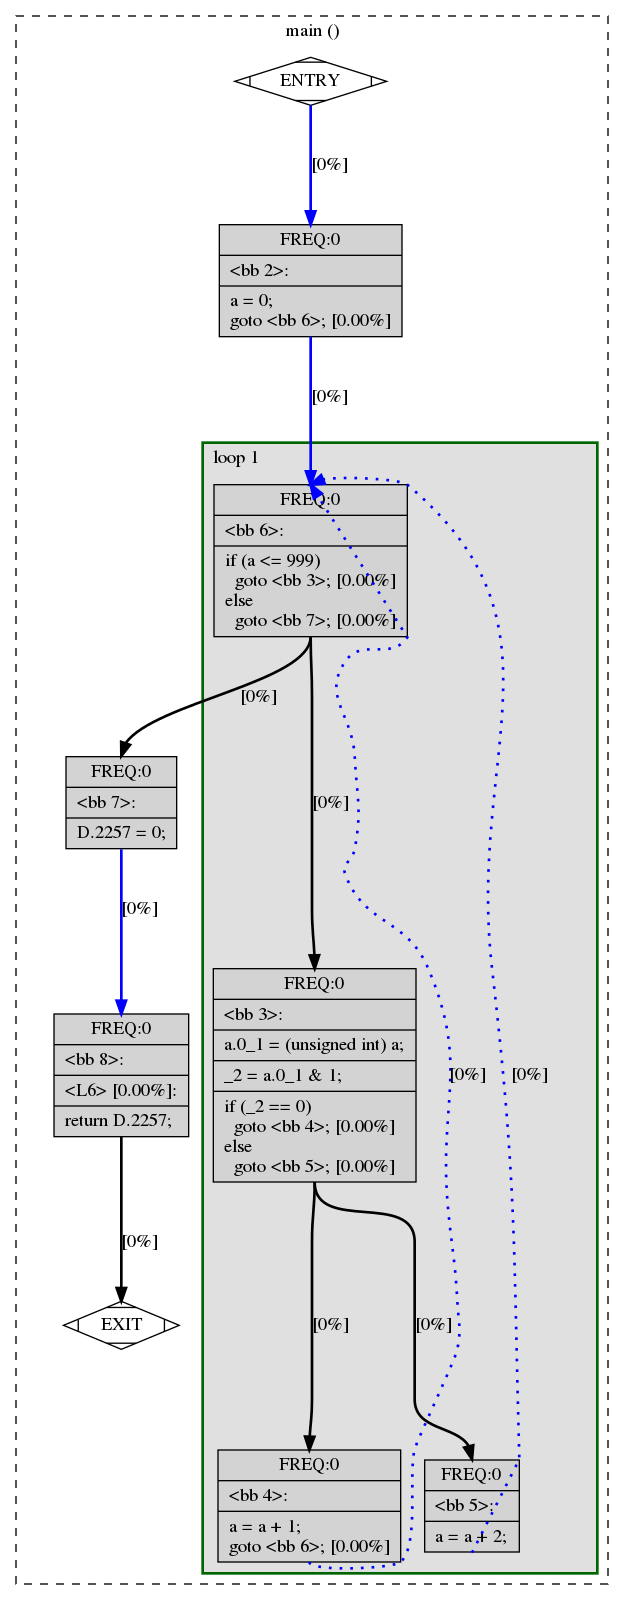
\includegraphics[scale=0.22]{images/graph.png}
    \captionof{figure}{Exemple CFG}
\end{center}
\end{multicols}
Comme l'exemple permet de le montrer, les graphes de flot de contrôle sont un excellent moyen de visualisation du code. Cependant sa véritable utilitée réside dans l'optimisation d'un code source.
\section{Nos recherches}

Afin d'étudier les Control Flow Graph, nous avons effectué un travail de recherche permettant de comprendre la modélisation des CFG, leur utilité et d'utiliser GCC pour générer et analyser des CFG. 

\subsection{Modélisation des CFG}
Nous allons dans un premier temps présenter la modélisation des CFG qui est déjà bien défini sur Wikipédia \cite{wiki:Graphe_de_flot_de_controle} mais approfondi dans la bible des compilateurs \cite{compilateurs}.

Les CFG font partis de la catégorie des graphes orientés. Cela signifie que ce sont des graphes dont les noeuds sont reliés par des arcs qui ont une direction. Les fonctions sont représentées par des sous-graphes disjoints les uns des autres.

Chaque noeud dans un CFG représente une portion de code, appelée \textbf{Bloc de base} dans laquelle il n'y a pas de saut ou de cible de saut. Un saut est défini par l'instruction \textit{goto xx} qui provient du langage assembleur et signifie \og saute à l'instruction xx \fg{}. L'entrée d'un bloc de base est la cible d'un saut, et la sortie est un saut.


Pour chaque fonction il existe toujours au moins deux blocs spéciaux. Le bloc \textit{Entry} qui caractérise l'entrée dans la fonction et donc le départ du flot, ainsi que le bloc \textit{Exit} qui caractérise la sortie de la fonction et la fin du flot.

Par construction le degré entrant et sortant d'un noeud, à part pour les blocs spéciaux définis ci-dessus, sont toujours supérieurs ou égaux à 1. En effet, si un bloc de base n'a pas de degré entrant, ce bloc n'est jamais exécuté et représente donc du code mort. Il peut alors être supprimé. De même, le seul bloc ayant un flot sortant nul est le bloc de sortie. 

Le code:
\begin{lstlisting}[language=c, numbers=left, xleftmargin=.35\textwidth, caption={Exemple de code à transformer}, captionpos=b]
    a = 0
    b = a + 70
    if b < 50
        print("Je ne vais pas afficher a")
        goto 7
    print(a)
    fin
\end{lstlisting}
se traduit en 4 blocs de base:
\newpage
\begin{lstlisting}[language=c, xleftmargin=.26\textwidth, caption={Séparation du code précédent en blocs de base}, captionpos=b]
    a = 0
    b = a + 70
    if b < 50

    print("Je ne vais pas afficher a")
    goto 7

    print(a)

    fin
\end{lstlisting}
et le graphe est représenté de la manière suivante:
\begin{center}
    \begin{tikzpicture}[
        node distance = 12mm and 6mm,
        box/.style = {rectangle, draw, fill=#1, 
                    minimum width=12mm, minimum height=7mm}
                    ]
        \node (n1) [box=white, align=justify] {a = 0\\b = a + 70\\if b < 50};
        \node (n2) [box=white, align=justify, below =of n1] {print("Je ne vais pas afficher a")\\goto 7};
        \node (n3) [box=white,below right=of n2] {print(a)};
        \node (n4) [box=white, below left=of n3] {fin};
        %
        \draw[->] (n1) to (n2);
        \draw[->, bend left] (n1) to (n3);
        \draw[->] (n2) to (n4);
        \draw[->] (n3) to (n4);
    \end{tikzpicture}
    \captionof{figure}{Graphe de blocs de base}
\end{center}

Les boucles introduisent un nouveau type d'arc: les \textit{arcs en arrière}. Ce sont des arcs spéciaux qui permettent de remonter à un arc déjà rencontré. En effet, un programme est exécuté ligne par ligne sauf lorsqu'une boucle fait explicitement remonter le programme à des instructions précédentes. 

Une boucle est constitué en en-tête d'un bloc \textbf{dominant} de la boucle qui représente sa condition et qui est la cible de l'arc en arrière. Ensuite ce bloc d'en-tête pointe vers la sortie de la boucle et vers le premier bloc de base de la boucle.

Voici un exemple:
\begin{lstlisting}[numbers=left, language=c, xleftmargin=.35\textwidth, caption={Exemple de boucle}, captionpos=b]
    a = -3
    while a > 0:
        a++
        goto 2
    print("sortie de boucle")
\end{lstlisting}

\begin{center}
    \begin{tikzpicture}[
        node distance = 12mm and 6mm,
        box/.style = {rectangle, draw, fill=#1, 
                    minimum width=12mm, minimum height=7mm}
                    ]
        \node (n1) [box=white, align=justify] {a = -3};
        \node (n2) [box=white, align=justify, below =of n1] {if a > 0};
        \node (n3) [box=white, align=justify, below =of n2] {a++\\goto 2};
        \node (n4) [box=white,below left=of n2] {print("sortie de boucle")};
        %
        \draw[->] (n1) to (n2);
        \draw[->] (n2) to (n3);
        \draw[->] (n2) to (n4);
        \draw[->, dashed, out = -40, in =40, looseness=2] (n3.south) to (n2.north);
    \end{tikzpicture}
    \captionof{figure}{Exemple graphe avec une boucle}
\end{center}

Les CFG permettent également d'étudier le flot du programme c'est à dire de savoir de quelle manière l'exécution a tendance à s'effectuer. Si par exemple une condition a plus souvent une chance d'être vraie ou fausse, une boucle de se terminer ou non. Cela a des utilités pratiques pour le compilateur comme nous allons l'évoquer dans la prochaine section.

\subsection{Utilité des CFG}
Lors de la compilation, le code source subit plusieurs analyses et opérations \cite{compilateurs}:
\begin{itemize}
    \item \textbf{Le prétraitement:} En langage C par exemple, il existe des instructions pour le préprocesseur qui permettent de créer des macros et des compilations conditionnelles. Le prétraitement va se charger de remplacer les macros et de gérer la compilation condtionnelle.
    \item \textbf{L'analyse lexicale:} Le code est passé sous découpe laser afin de l'écrire sous forme de \textit{jetons} (ou \textit{tokens} en anglais) qui représentent les mots clef du langage, identifiants et symboles. 
    \item \textbf{L'analyse syntaxique:} Analyse de la suite des jetons afin de construire un arbre basé sur la grammaire du langage. Par exemple, une boucle contient toujours une condition.
    \item \textbf{L'analyse sémantique:} L'arbre précédemment construit reçoit des informations sémantiques. Durant cette phase, le compilateur vérifie le type des variables, construit la table des symboles (qui contient les identifiants des variables, leur \textit{scope}, ...).
    \item \textbf{Génération du code intermédiaire:} L'arbre est utilisé pour générer un code dit intermédiaire qui permet de réaliser des opérations plus aisées d'optimisation.
    \item \textbf{Optimisation du code intermédiaire:} Le code intermédiaire est optimisée afin de soit modifier le code pour le rendre plus efficace (exemple: suppression de variables inutiles par propragation de constante), ou supprimer du code mort détecté.
    \item \textbf{Génération du code:} Dernière étape durant laquelle, l'exécutable est créé.
\end{itemize}
Il est à noter que ces phases ne sont ni nécessairement linéaires, ni uniques. Le compilateur effectue des opérations parallèles entre différentes portions du code et des passes afin d'optimiser plusieurs fois le code généré.

Les CFG dans ces étapes d'optimisation servent à plusieurs choses. Tout d'abord, détecter du code mort car comme il a été dit en introduction, si un bloc de base n'a pas de degré entrant, alors il n'est jamais exécuté.

De plus, il est parfois utile de savoir quelle est la probabilité qu'un code soit exécuté afin que le compilateur privilégie une exécution plus rapide d'une branche plutôt qu'une autre. La documentation GCC évoque plus en détail cette étape \cite{gcc:cfg}.

Cependant, les CFG ne sont pas seulement utiles pour le compilateur, mais pour de nombreux analyseurs statiques. Il permet de connaitre l'ordre d'exécution d'un programme par sa construction en arbre, d'étudier si un programme / une fonction contient des boucles, la résilience d'un programme... Beaucoup d'analyse basée sur la théorie des graphes peuvent être effectués afin d'étudier la structure du code source à partir de sa représentation en graphe.

\subsection{Outil de GCC}
Afin de nous permettre d'étudier et de comprendre les CFG, nous avions besoin d'avoir un outil permettant de les générer. GCC via sa palette d'options de compilation nous a fourni cet outil. Par exemple via GCC\footnote{Commande Bash utilisée: \textbf{gcc -fdump-tree-all-graph <target.c>}}, le code et son graphe ci-dessous:
\begin{multicols}{2}
\lstinputlisting[language=c, caption={Exemple de code avec une boucle pour transformation en CFG}, captionpos=b]{code/code.c}
\begin{center}
    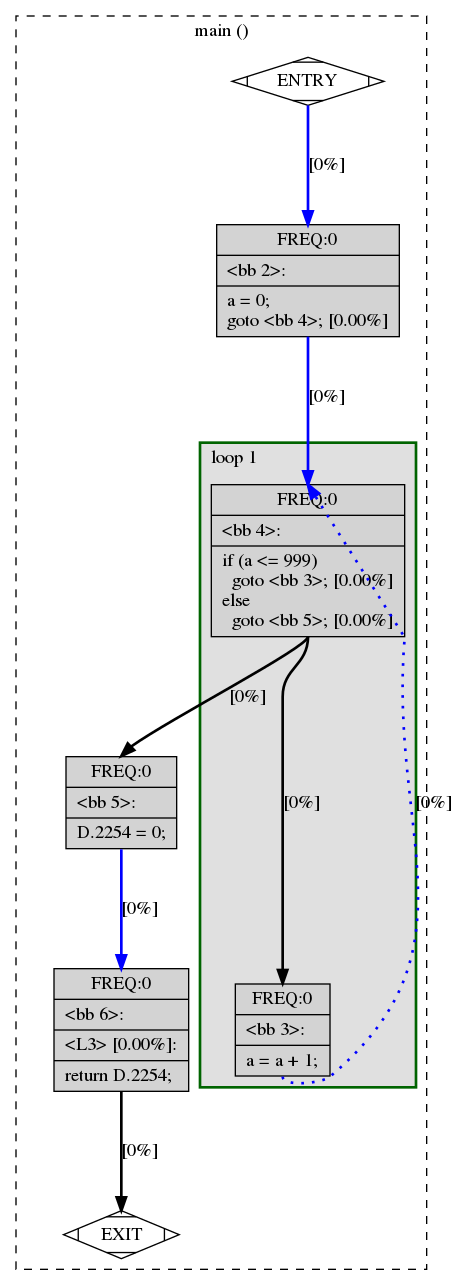
\includegraphics[scale=0.3]{images/graph2.png}
    \captionof{figure}{CFG généré avec le code précédent}
\end{center}
\end{multicols}
\section{Implémentation}
Dans le cadre de notre étude des CFG, nous avons réalisé deux scripts différents via l'utilisation de python et de différentes librairies.

Comme nous avons pu le voir, grâce à GCC, nous avons pu générer des CFG. Pour pouvoir avoir une représentation adéquate, GCC propose un fichier de sortie au format \textit{.dot}\footnote{Le langage DOT est un langage de description de graphe dans un format texte.}.

\subsection{Notre script de modifications des CFG}
De base, lorsqu'un CFG est généré, les fonctions sont séparées dans des sous graphes distincts. Cela est intéressant car il est alors possible d'analyser chacune des fonctions séparémment, ce qui est en générale l'intérêt d'une fonction, encapsuler du code.

Cependant, l'intérêt d'un CFG, c'est aussi de savoir comment le flot traverse le programme. Or, il peut-être intéressant de voir le flot entre deux fonctions. Nous avons donc développé un script permettant de raccorder deux fonctions lorsque celles-ci sont situées dans le même fichier.

Prenons l'exemple du code source suivant:
\lstinputlisting[language=c, xleftmargin=.35\textwidth, caption={Programme d'exemple pour le script de modifications}, captionpos=b]{code/cfg_avant.c}

\pagebreak
Le CFG fabriqué à partir de ce code par GCC est ceci:
\begin{center}
    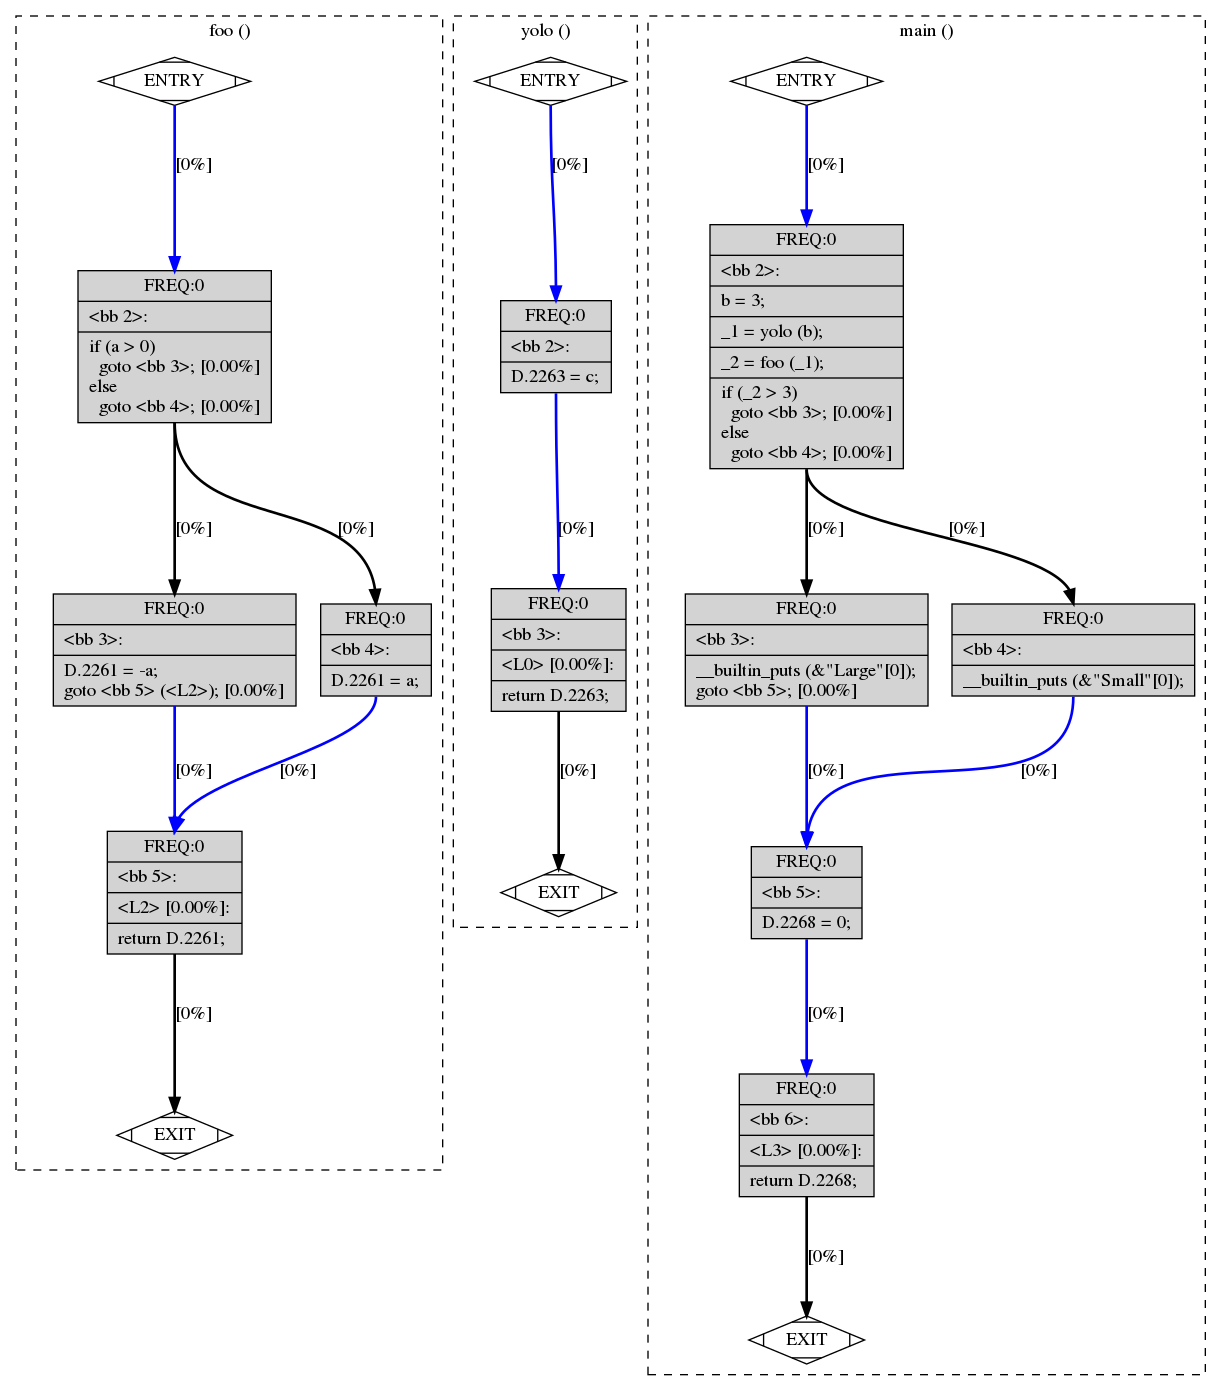
\includegraphics[scale=0.32]{images/cfg_avant.png}
    \captionof{figure}{CFG avant utilisation du script}
\end{center}
Comme il est possible de le constater dans le code et le CFG, les appels à fonction sont identifiables dans ce programme et après passage du fichier dot représentant ce graphe dans notre script, voici le nouveau CFG que nous avons obtenu:
\begin{center}
    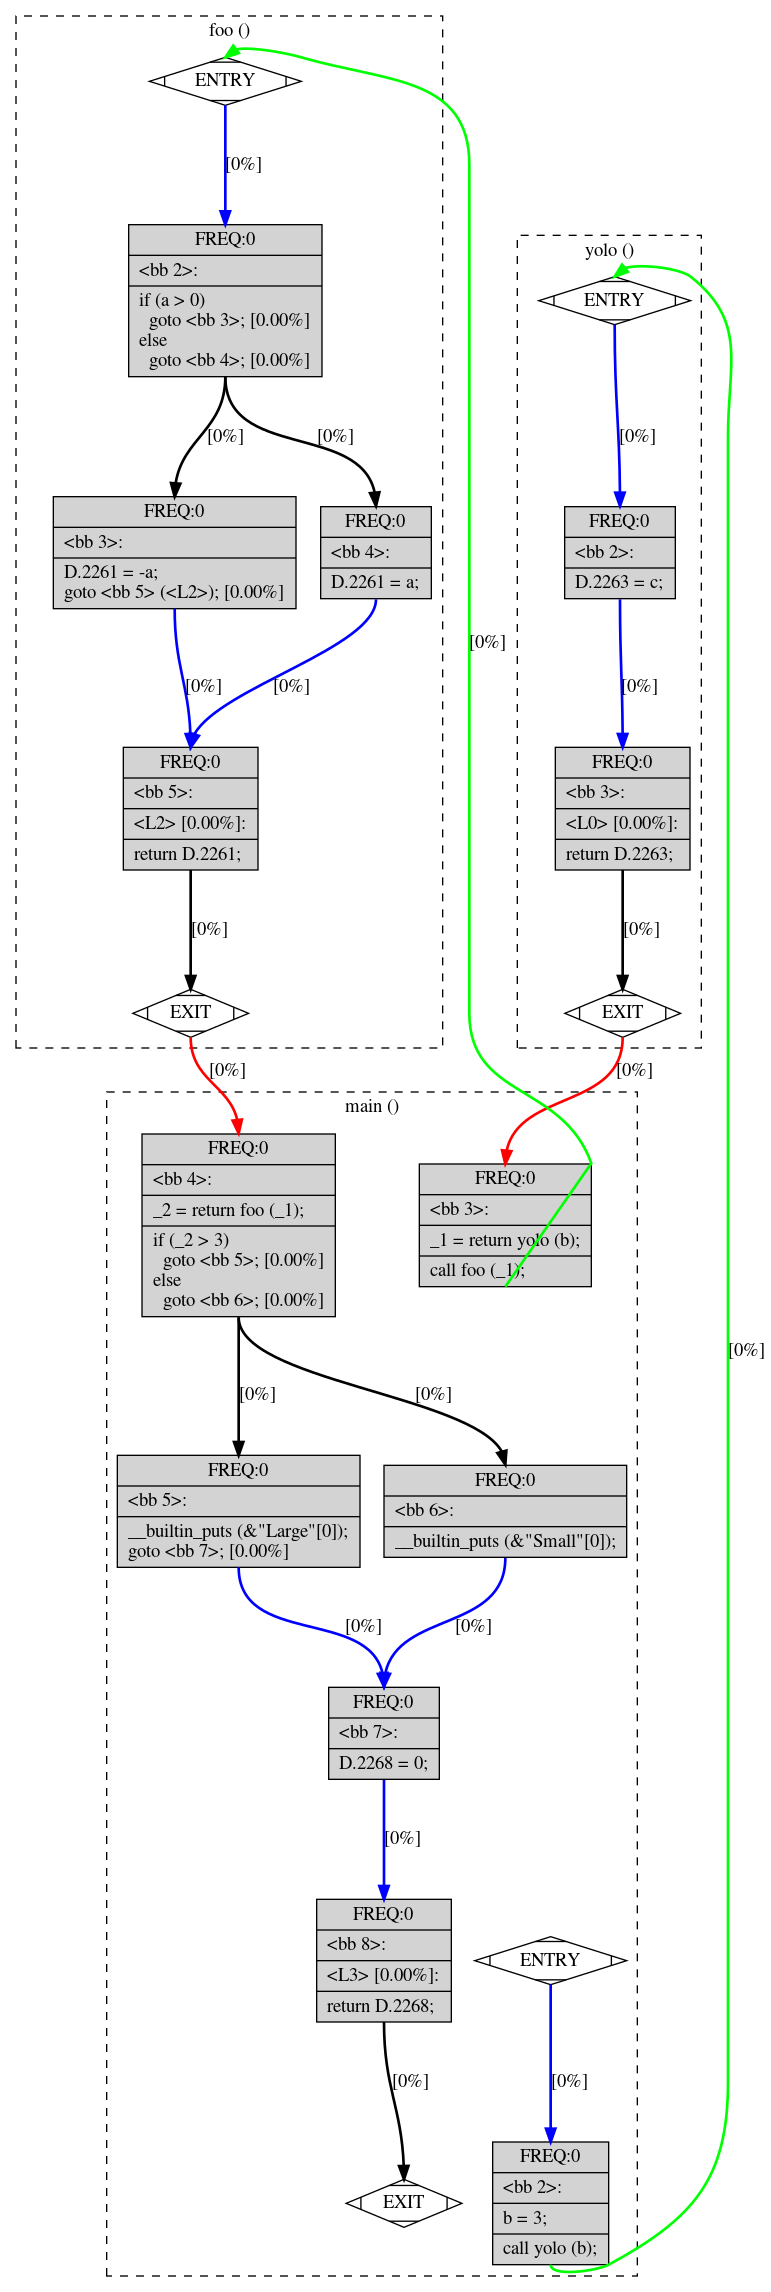
\includegraphics[scale=0.24]{images/cfg_apres.png}
    \captionof{figure}{CFG après utilisation du script}
\end{center}
Pour ce faire, nous avons utilisé une librairie appelée \textit{pydot}\footnote{Pydot est une librairie pouvant parser du code DOT généré par la librairie GraphViz (utilisée par GCC pour générer des CFG).} qui nous a permis de parser les fichiers DOT et de les modifier par le langage de programmation Python.

Nous avons décidé que les blocs de base spéciaux \textit{Entry} et \textit{Exit}, seront désormais des blocs normaux avec un flot entrant et sortant, sauf pour l'entrée et la sortie du programme. Les appels à fonctions sont désormais considérés comme des sauts et la variable de retour est la cible du saut de la fin de fonction, ce qui permet de définir deux nouveaux blocs de base à partir d'un appel à fonction.

On remarque que le flot passe maintenant dans les fonctions ce qui permet de mieux les situer les unes par rapport aux autres. Cela permet notamment d'identifier du code mort ou non utile dans le fichier parsé. En effet, si on remarque qu'une fonction n'est pas atteinte, cela signifie que son code n'est jamais exécutée (par les fonctions présentes dans son fichier).

\subsection{Notre script d'analyse des CFG}
Nous avons développé un second script permettant d'analyser les CFG en utilisant encore une fois Python et une librairie nommée \textit{NetworkX}\footnote{NetworkX est une librairie permettant de modéliser, analyser la structure et la dynamique de graphe via un lot de fonctions implémentées.}. Notre script permet d'analyser différentes choses.

Il identifie quels sont les noeuds qui n'ont pas de degré entrant, ce qui signifie qu'il est capable de détecter du code mort au sens du fichier, c'est à dire, si une fonction n'est pas exécutée par une autre dans un fichier. Il peut également détecter si un graphe est acyclique, c'est à dire si une boucle est présente ou non dans un graphe.

Le script renvoie également le plus court et long chemin entre le début et la fin du graphe (donc du programme) ce qui permet d'étudier quelles sont les différentes étapes d'exécution qui entraine une durée plus ou moins importante du programme.

Il permet également d'étudier la connectivité qui représente le nombre de possibilité moyenne pour aller d'un noeud à un autre. Plus ce nombre est haut, plus il y a de conditions dans le programme.

Pour le CFG de la section précédente après traitement par notre script de modifications des appels à fonction, le script d'analyse renvoie les résultats suivants:
\begin{itemize}
    \item Il y a un noeud sans entrée dans la fonction main, ce qui correspond à l'entrée du programme.
    \item Les chemins plus long et court font 17 noeuds.
    \item Le graphe est acyclique.
    \item Le graphe a une connectivité de 1.19.
    \item Il n'y a pas de noeuds isolés.
\end{itemize}
Analysons maintenant le graphe généré par notre programme:
\lstinputlisting[language=c, xleftmargin=.35\textwidth, caption={Exemple de code pour le script d'analyse}, captionpos=b]{code/fonction_inutile.c}

Le graphe est alors:
\begin{center}
    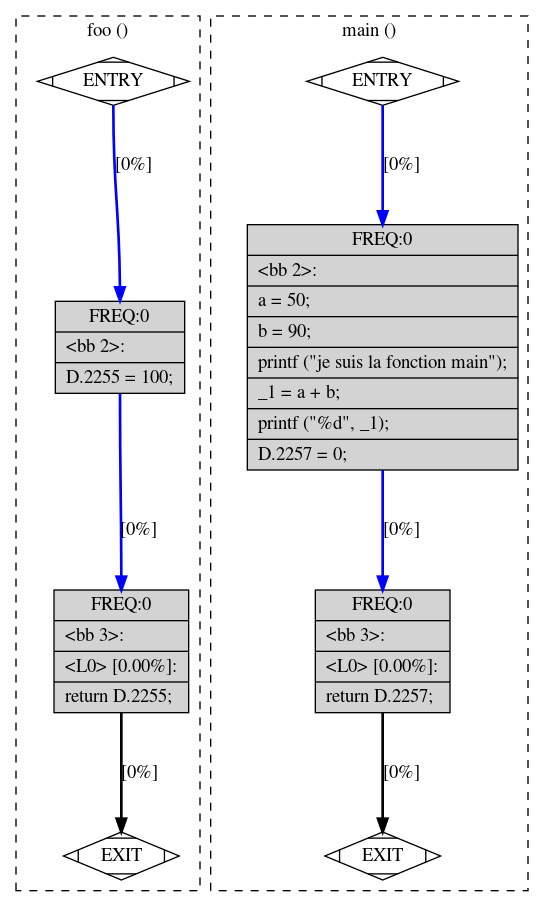
\includegraphics[scale=0.35]{images/fonction_inutile.png}
    \captionof{figure}{CFG pour le script d'analyse avant utilisation du script de modifications}
\end{center}

Notre script d'analyse renvoie ceci:
\begin{itemize}
    \item Il y a un noeud sans entrée dans la fonction foo
    \item Il y a un noeud sans entrée dans la fonction main
    \item Les chemins plus long et court font 4 noeuds.
    \item Le graphe est acyclique.
    \item Le graphe a une connectivité de 1.
    \item Il n'y a pas de noeuds isolés.
\end{itemize}
On remarque donc que notre script a bien détecté qu'une fonction n'est jamais exécutée et donc qu'il y a du code mort. Le degré de connectivité a également baissé, ce qui est logique car il y a moins de chemins puisqu'il n'y a pas de conditions. Il n'y a toujours pas de noeuds isolés car la fonction foo contient plusieurs noeuds.
\chapter{Dead Code Detection}
\section{Introduction}
La détection de code mort est une branche importante d'optimisation en informatique. Le code mort se définit ainsi:
\begin{quotation}
    Code qui n'est jamais exécuté, ou dont le résultat n'est jamais exploité par son programme.
    \footnote{Wikitionary: \url{https://fr.wiktionary.org/wiki/code_mort}.}
\end{quotation}
Le code qui n'est jamais exécuté représente plusieurs inconvénients. D'abord, il prend inutilement de la place en mémoire pour des raisons évidentes. De plus, du code mort causé par une condition peut représenter un temps plus long d'exécution du programme.

Voici un exemple de suppression de code mort:
\begin{multicols}{2}
\begin{lstlisting}[language=c]
    int main() {
        int a = 0;
        int b = -150000;
        
        while (b < a) {
            if(b < a) {
                ...
            } else {
                :::
            }
            b++;
        }
    
        return 0;
    }
\end{lstlisting}
\columnbreak
\begin{lstlisting}[language=c]
    int main() {
        int a = 0;
        int b = -150000;
        
        while (b < a) {
            ...
            b++;
        }
    
        return 0;
    }
\end{lstlisting}
\end{multicols}
\begin{center}
    \captionof{lstlisting}{Le code a gauche contient du code mort, à droite il est optimisé}
\end{center}

On remarque que le programme de droite est non seulement plus court, mais évite également 150.000 qu'une condition soit vérifiée. De nombreux compilateurs et analyseurs syntaxiques permettent de détecter du code mort, GCC par exemple aurait détecté le code mort précédent et aurait réarrangé le code durant la compilation pour le supprimer.

\section{Nos recherches}
\subsection{Des exemples de détection de code mort}
A l'heure actuelle, la détection de code mort via des outils d'analyseurs syntaxique est très performante pour des cas spécifiques. En effet des cas usuels simples sont déjà traités. Par exemple prenons le code suivant:
\begin{lstlisting}[language=c, xleftmargin=.25\textwidth, caption={Exemple de programme avec du code mort}, captionpos=b]
    int main() {
        int a = 0;
        int b = -150000;
        
        while b < a) {
            if(b < a) {
                ...
            } else {
                :::
            }
            b++;
        }
    
        return 0;
        printf("Je suis du code mort\n");
        printf("En dessous du return.\n");
    }
\end{lstlisting}

Les compilateurs modernes signaleront ou supprimeront le code mort situé en dessous de l'instruction return. En effet, les printf ne seront jamais exécutés puisque le return annonce la fin de la fonction.

Un autre exemple est la propagation de constante \cite{compilateurs}, c'est à dire le remplacement des variables par leur valeur losqu'elles sont connues, qui permet de supprimer du code mort de façon assez importante. En effet, le compilateur effectue plusieurs passes sur le code pour remplacer les variables par leur valeur si elles sont connues, et évaluent ensuite les conditions si elles peuvent l'être.
\newpage
En voici un exemple en trois temps:
\begin{multicols}{3}
    \begin{lstlisting}[language=c]
        int main() {
            int a = 0;
            int b = 1;
            
            if(b < a){
                ...
            } else {
                :::
            }
        
            return b;
        }
    \end{lstlisting}
    \columnbreak
    \begin{lstlisting}[language=c]
        int main() {
            
            if(1 < 0){
                ...
            } else {
                :::
            }
        
            return 1;
        }
    \end{lstlisting}
    \columnbreak
    \begin{lstlisting}[language=c]
        int main() {

            :::
        
            return 1;
        }
    \end{lstlisting}
\end{multicols}
\begin{center}
    \captionof{lstlisting}{De gauche à droite, propagation de constante après 0, 1, 2 passes du compilateur}
\end{center}
En faisant de nombreux tests de suppresion de code mort grâce à GCC en demandant au compilateur de créer un fichier en code assembleur optimisé le plus possible, nous nous sommes rendus compte qu'il y a une détection de code \og potentionnelement mort \fg{} qui n'est pas effectué.

Le code suivant, déclarant une fonction foo dont le fonctionnement ne nous intéresse pas, n'est pas nécéssairement optimisé:
\begin{lstlisting}[language=c, xleftmargin=.2\textwidth, caption={Exemple de programme avec du code potentiellement mort}, captionpos=b]
    int main(const int a, const unisgned int d) {
        int b = a + d;
        
        if(b < a) {
            ...
        } else {
            +++
        }
        return 0;
    }
\end{lstlisting}
En effet dans un monde purement mathématiques, nous avons que $a + d = b > a$ car $d > 0$. Cependant en informatique les valeurs infinies n'existent pas et si un entier est supérieur à la valeur maximale, via un modulo, l'entier a une valeur inférieur à celle escomptée. Cela s'appelle \og l'arithmétique modulo\footnote{Cet article wikipédia explique très bien comment fonctionne cette arithmétique: \url{https://fr.wikipedia.org/wiki/Congruence_sur_les_entiers}.}\fg{}.

Ainsi le compilateur n'a pas optimisé le code car il ne sait pas si le développeur prend en compte ou non cette notion d'arithmétique ou s'il a simplement commis une erreur de programmation, ce que nous appelons donc du code \og potentionnelement mort \fg{}.

\subsection{La détection d'incohérence}

Après avoir découvert la possibilité de détecter du code \og potentionnelement mort \fg{}, nous avons décidé d'étudier si des techniques actuelles permettraient de pouvoir effectuer une analyse du code prenant en compte cette possibilité.

Nous nous sommes intéressé à un problème équivalent plutôt utilisé en test dénommé la détection d'incohérence ou "Inconsistency detection". Nous avons trouvé en particulier une thèse informatique qui traite le problemme de détection d'incohérence en étudiant la possibilité d'atteindre une instruction d'un programme en fonction de conditions qui sont évaluées successivement vraies ou fausses dans des branches différentes \cite{inconsistencies}.

Pour bien comprendre comment cela fonctionne, prenons un exemple avec le code suivant:
\begin{lstlisting}[language=c, xleftmargin=.2\textwidth, caption={Programme d'exemple pour la détection d'incohérence}, captionpos=b]
    int foo(int a, int b){
        int mid = (a + b) / 2;
        if(a <= b) {
            return mid;
        } else if(a == b) {
            return a;
        } else if(a > b) {
            return b;
        }
    }
\end{lstlisting}
Il y a ici trois résultats, donc trois branches, possibles à l'évaluation d'une condition. Prenons arbitrairement la branche qui vérifie que la deuxième branche est évaluée à true. On aurait ceci:
\begin{lstlisting}[language=c, xleftmargin=.2\textwidth, caption={Deuxième branche évaluée à true du programme}, captionpos=b]
    int mid = (a + b) / 2;
    assume(a > b);
    assume(a == b);
    return a;
\end{lstlisting}
On remarque que cette branche est impossible, en effet, il n'est pas possible que $a > b$ et $a == b$. La détection d'incohérence consiste donc à créer deux ou plus contextes d'évaluation à chaque fois qu'une condition est rencontrée. Ensuite chaque contexte prend en compte cette condition et vérifie si elle est en accord avec les précédentes conditions rencontées. Par exemple ce code, que GCC n'optimise pas comme vu précédemment, contient une incohérence:
\begin{lstlisting}[language=c, xleftmargin=.2\textwidth, caption={Exemple d'incohérence non optimisé par GCC}, captionpos=b]
    int main(const int a, const unisgned int d) {
        int b = a + d;

        if(b > a) {
            ...
        } else {
            +++
        }

        return 0;
    }
\end{lstlisting}
En effet, pour la raison expliquée précédemment mathématiquement on a $b > a$ et donc la branche else ne peut jamais être prise.

\subsection{Analyse de valeurs}
L'analyse de valeurs, ou \og Value Analysis \fg{} consiste à associer pour chaque variable dans un programme les valeurs qu'il est possible pour elle d'atteindre à chaque point de ce programme.

Nous nous sommes intéressés à cette branche de recherche, car il nous est venu à l'esprit qu'il serait possible d'améliorer la détection d'incohérence en ajoutant l'analyse de valeurs dans les contextes d'évaluation des conditions afin de détecter les incohérences dûes aux valeurs. Voici un exemple:
\begin{lstlisting}[language=c, xleftmargin=.15\textwidth, caption={Exemple d'incohérence détectable par Value Analysis}, captionpos=b]
    int main(const int a, const unisgned int d) {
        int b = a + d;
        int w = a - d

        if(b < w) {
            ...
        } else {
            :::
        }

        return 0;
    }
\end{lstlisting}
En prenant en compte l'analyse de valeurs, on se rend compte, en ommettant l'arithmétique modulo, que $b$ est nécessairement supérieur à $w$ et donc que le contexte prenant la branche else est nécessairement fausse.

\section{Implémentation}
Nous avons décidé de créer un script Python permettant de détecter les incohérences dans des contextes d'évaluation de conditions en pratiquant l'analyse de valeurs sur des programmes en language C.

Afin de pouvoir développer un prototype, nous avons décidé de poser plusieurs restrictions:
\begin{itemize}
    \item Travailler avec uniquement des entiers
    \item Travailler avec des additions
    \item Les conditions sont seulement des opérations avec les opérateurs $<$ et $>$
    \item Une variable doit seulement dépendre d'une autre variable et d'une constante. C'est à dire que si $a$ est un paramètre de fonction, elle peut valoir toutes les valeurs et $b = a + 1$ peut valoir toutes les valeurs. Par contre $b = a + d$ et $d$ n'importe quelle variable n'est pas une opération autorisée.
\end{itemize}

Ce script utilise la bibliothèque Pycparser\footnote{Pycparser est un parser du langage C qui permet de récupérer le graphe AST du programme parsé.}.
\newpage
Voici le pseudo code du script qui analyse une fonction:
\begin{lstlisting}[numbers=left, caption={Pseudo code du script de détection d'incohérence}, captionpos=b]
    Creer le graphe a partir d'une fonction passee en parametre
    context = creation du contexte de base
    Pour chaque variable en parametre de la fonction:
        Ajouter la variable au contexte avec la valeur: [-inf, inf]
    Pour chaque noeud du graphe
        Pour chaque contexte:
            Pour chaque noeud du graphe dans la liste des noeuds du contexte:
                Si le noeud est une declaration de variable:
                    Ajouter la variable au contexte avec la valeur d'initialisation
                Sinon si le noeud est une assignation de variable:
                    Mettre a jour la valeur de la variable
                Sinon si le noeud est une condition:
                    Creer deux contextes c1 et c2 heritant du contexte actuel
                    Donner l'evaluation true de la condition a c1
                    Donner l'evaluation false de la condition a c2
                    Si la condition pour c1 n'est pas possible, stopper c1
                    Si la condition pour c2 n'est pas possible, stopper c2
                    Faire parcourir la branche true a c1
                    Faire parcourir la branche false a c2
    Afficher les contextes ayant ete stoppes avec le numero de ligne en cause
\end{lstlisting}

Ainsi le script issu de ce pseudo code renvoie les contextes ayant été stoppés car la condition dans un contexte d'évaluation n'a pas pu être évaluée à $False$ ou à $True$ ce qui signifie que soit la condition est toujours vraie, soit la condition est toujours fausse et donc qu'il y a du code mort potentiellement mort.

Notre ambition aurait été de pouvoir ajouter ce script à un éditeur de code comme VS Code\footnote{Visual Studio Code est un éditeur de code facilement modulable gratuit et opensource qui a été développé par Microsoft et est cross-platform.}, afin d'aider les développeurs à pouvoir analyser leur code et ainsi repérer si des conditions sont inutiles et donc si soit ils n'avaient pas vu que la condition était toujours vraie, ou s'il avaient effectué une erreur de programmation.

Malheuresement, avec le temps du projet Cassiopée, nous n'avons pas pu terminé l'implémentation du script même avec les restrictions que nous nous étions imposés. 

Cependant, nous considérons que nous avons rencontré le but de ce projet, qui était d'étudier la structure du code d'un programme et trouver si des optimisations étaient possibles. Il se trouve que notre idée de script n'a pas encore été implémenté à notre connaissance, en effet, aucun des éditeurs de code que nous avons utilisé ne nous a jamais averti via des warning de ce genre d'incohérences. Nous pensons donc que c'est une piste intéressante de développement qui pourrait aider les développeur à améliorer leur processus de correction de code. En effet, même si un développeur avait pris en compte l'arithmétique modulo, nous considérons que le taux de \og false positives \fg{} générés par le script resterait bien inférieur au taux de \og true positives \fg{}.

\bibliographystyle{unsrt}
\bibliography{rapport}

\end{document}